% =====================================================================================================
\section{Conjunto de missões}\label{sec:dataset}

Um benchmark de alocação só é útil se as suas missões se parecerem com ataques reais. Os cenários da literatura costumam
ser sintéticos: alvos e rotas sorteados no mapa e, muitas vezes, radares posicionados para cobrir as rotas do próprio
ataque --- o que dá ao defensor um conhecimento que ele não teria. Construímos as missões a partir de três fontes de
realismo: \emph{onde} se ataca (ativos reais de infraestrutura sobre o relevo real), \emph{com o quê} se ataca (classes
de ameaça com parâmetros de fontes abertas) e \emph{como} se ataca (eixo de ameaça, rotas que aproveitam o relevo,
iscas e chegada coordenada). A defesa, por sua vez, é montada sem conhecer o ataque.

\subsection{Cidades e ativos}
As missões cobrem seis cidades: São José dos Campos, Taubaté e Itajubá, polos aeroespacial, industrial e de energia do
Vale do Paraíba e do sul de Minas Gerais, e as três maiores concentrações de infraestrutura e de governo do país, São
Paulo, Rio de Janeiro e Brasília. Cada mapa tem 12 a 14~km de lado, sobre o modelo de elevação Copernicus
GLO-30~\cite{copernicusDEM}; os relevos vão do planalto quase plano de Brasília às serras do Vale e aos maciços do Rio,
o que produz desde regiões de boa cobertura de radar até sombras extensas atrás dos morros.

Os \conceito{ativos} --- os alvos possíveis --- são extraídos do OpenStreetMap~\cite{osm}: usinas e aeródromos
(importância 4), subestações, estações de tratamento de água e esgoto e áreas industriais de mais de 50~ha (importância
3), torres de telecomunicação e áreas industriais de 5 a 50~ha (importância 2). Entre 31 (Itajubá) e 329 (São Paulo)
ativos por cidade. A extração é gravada junto com o código, de modo que as missões não mudam se o mapa colaborativo mudar.

Em cada missão, de dois a três ativos são \conceito{defendidos}: viram zonas prioritárias, com raio igual ao do ativo
mais 250~m (entre 300 e 1000~m). Eles são sorteados em dois passos --- primeiro a categoria, com peso proporcional ao
cubo da importância, depois o ativo dentro dela, favorecendo os maiores ---, para que as dezenas de torres de uma cidade
não dominem a escolha só por serem numerosas. Nas 192 missões, os ativos defendidos são estações de água (109),
subestações (99), aeródromos (90), áreas industriais (80), usinas (74) e torres de telecomunicação (28).

\subsection{Defesa}
A defesa é montada a partir dos ativos defendidos, \emph{sem conhecer o ataque}. De quatro a sete radares são postos nos
topos de morro que mais cobrem a área até 5~km de cada ativo defendido, escolhidos de forma gulosa, com sorteio entre os
três melhores a cada passo. Há uma base de interceptadores a 0,8--2~km de cada ativo defendido e, às vezes, uma base
central, com $\lceil 1{,}25N\rceil$ interceptadores no total --- uma folga de 25\,\% sobre o número de ameaças, que precisa
cobrir também os interceptadores gastos com falsos alarmes e iscas. Ao contrário de um gerador que posiciona os radares
para cobrir as rotas do ataque, nenhuma missão é descartada por cobertura: a fração das rotas coberta pelos radares, a
120~m sobre o terreno, varia de 38 a 100\,\% e é uma característica da missão, não um critério de seleção.

\subsection{Classes de ameaça}
A Tabela~\ref{tab:classes} resume as quatro classes. As velocidades e alturas vêm de fontes abertas sobre os vetores
empregados na guerra na Ucrânia: o drone de ataque de longo alcance do tipo Shahed-136/Geran-2, que voa a 150--185~km/h
numa rota pré-programada e usa tanto alturas muito baixas, para se esconder no relevo, quanto alturas de vários
quilômetros~\cite{gurShahed,gsGeran2,dwShahed}; a isca do tipo Gerbera, mais barata, de assinatura de radar parecida ou
ampliada, lançada junto com os drones de ataque para atrair a defesa --- numa proporção relatada de cerca de 40\,\% da
onda~\cite{isisGerbera,capssGerbera,dnGerbera}; a munição vagante do tipo Lancet-3, de 80--110~km/h, que orbita sobre o
alvo e mergulha a cerca de 300~km/h~\cite{gdLancet,gsLancet}; e o drone FPV de ataque, que em combate voa a 60--80~km/h,
com máximo de cerca de 120~km/h~\cite{kyivpostFPV}. A seção radar, o valor de dano e a inclinação do mergulho são
hipóteses do modelo; o valor de dano é aproximadamente proporcional, de forma comprimida, à carga explosiva.

\begin{table}[t]
\centering
\caption{Classes de ameaça. Velocidade e altura de fontes abertas (ver texto); seção radar (RCS), valor de dano $\nu_a$
e mergulho são hipóteses do modelo. Mergulho: inclinação da rampa final até o impacto.}
\label{tab:classes}
\small
\begin{tabularx}{\textwidth}{@{}lXXcccX@{}}
\toprule
Classe & Velocidade & Altura sobre o terreno & Mergulho & RCS (m$^2$) & $\nu_a$ & Comportamento \\
\midrule
ataque & 42--51~m/s & 60--150~m (50\,\%) ou 500--1500~m & 45° & 0,3--1,0 & 1 & rota pré-programada \\
isca & 27--44~m/s & 80--200~m (70\,\%) ou 500--1200~m & raso & 0,5--1,5 & 0 & como o ataque; chega antes \\
vagante & 22--31~m/s & 300--800~m & 63° & 0,1--0,4 & 0,5 & orbita o alvo (400--700~m) e mergulha \\
FPV & 17--33~m/s & 20--50~m & raso & 0,02--0,1 & 0,25 & curvas aleatórias; metade reage ao interceptador \\
\bottomrule
\end{tabularx}
\end{table}

Toda missão mistura as quatro classes, em uma de quatro \conceito{composições} (Tabela~\ref{tab:composicoes}): de
\emph{saturação}, que segue a proporção relatada de iscas; de \emph{longo alcance}, dominada por drones de ataque;
\emph{tática}, dominada por munições vagantes e FPV; e \emph{equilibrada}. Cada classe tem pelo menos uma ameaça.

\begin{table}[t]
\centering
\caption{Composições do enxame: fração das ameaças em cada classe.}
\label{tab:composicoes}
\small
\begin{tabular}{@{}lcccc@{}}
\toprule
Composição & ataque & isca & vagante & FPV \\
\midrule
saturação & 45\,\% & 40\,\% & 10\,\% & 5\,\% \\
longo alcance & 60\,\% & 25\,\% & 10\,\% & 5\,\% \\
tática & 15\,\% & 10\,\% & 40\,\% & 35\,\% \\
equilibrada & 25\,\% & 25\,\% & 25\,\% & 25\,\% \\
\bottomrule
\end{tabular}
\end{table}

\subsection{Ataque}
\paragraph{Eixo de ameaça.} Um ataque real vem de uma direção, a do território de onde é lançado. Cada missão sorteia um
\conceito{eixo de ameaça} e um setor de 60 a 90°; as ameaças entram pela borda do mapa dentro desse setor, que pode girar
até 20° entre ondas. Como os mapas têm 12 a 14~km, só o trecho final das rotas de longo alcance é simulado.

\paragraph{Alvos.} Três quartos das ameaças armadas vão a um ativo defendido; as demais, a ativos não defendidos, cujo
impacto tem penalidade baixa ($w_O$). As iscas vão a ativos quaisquer. O ponto de impacto é sorteado dentro da área do
ativo.

\paragraph{Rotas sobre o relevo.} As rotas são caminhos de menor custo numa grade de 150~m, do ponto de entrada ao alvo,
com custo por célula $1+\beta\,\tilde h+0{,}6\,\xi$, em que $\tilde h$ é a altura do terreno normalizada no mapa, $\xi$
um ruído suave sorteado a cada missão (que torna as rotas diferentes entre missões) e $\beta$ depende da altura de voo:
$\beta=3$ para quem voa baixo, que passa a seguir os vales e a se esconder do radar atrás dos morros, e $\beta=0{,}3$
para quem voa alto, cuja rota é quase reta. Uma penalidade perto da borda evita rotas que correm rente a ela. A rota é
simplificada a um ponto de controle a cada 700~m e suavizada. As munições vagantes terminam com uma órbita completa
sobre o alvo antes do mergulho.

\paragraph{Chegada coordenada.} As ameaças entram em uma a três \conceito{ondas}, separadas por 120 a 300~s. Dentro de
cada onda, o instante de entrada de cada ameaça é calculado a partir do comprimento da sua rota e da sua velocidade
para que todas cheguem ao alvo num intervalo de 60~s --- de modo que vetores lentos e rápidos, vindos de pontos
diferentes, saturem a defesa ao mesmo tempo. As iscas chegam 30 a 90~s antes, para atrair os interceptadores.

\subsection{Aleatoriedade e delineamento}
Cada missão é um \emph{gerador} de episódios, e não uma situação fixa: a cada execução, os pontos de controle das rotas
(num raio de 100 a 250~m), as velocidades, as alturas, os pontos de entrada e os parâmetros das manobras são sorteados
de novo dentro das faixas da classe. Isso evita que um método aprendido decore situações específicas.

O \conceito{delineamento} é \emph{balanceado}: em cada cidade, cada combinação de tamanho do enxame,
$N\in\{12,24,36,48\}$, e composição aparece exatamente duas vezes, o que dá 32 missões por cidade e 192 no total, com
5760 ameaças (2004 drones de ataque, 1440 iscas, 1260 munições vagantes e 1056 FPV). Assim, tamanho, composição e cidade não
ficam confundidos e o efeito de cada fator pode ser medido separadamente. A semente de cada cidade é derivada do seu
nome, de modo que acrescentar ou retirar cidades não muda as missões das demais.

\subsection{Treino e teste}
As 64 missões do Rio de Janeiro e de Brasília formam o conjunto de \conceito{teste}: os métodos com parâmetros ajustados
a partir de dados (a árvore com utilidade e as redes neurais) usam só as 128 missões das outras quatro cidades, e são
avaliados em cidades que nunca viram --- com outro relevo, outros ativos e outro arranjo da defesa. Brasília, plana, e o
Rio, entre o mar e os maciços, são também os dois relevos mais diferentes dos do treino. A Figura~\ref{fig:cenario}
mostra uma missão de teste.

\begin{figure}[t]
\centering
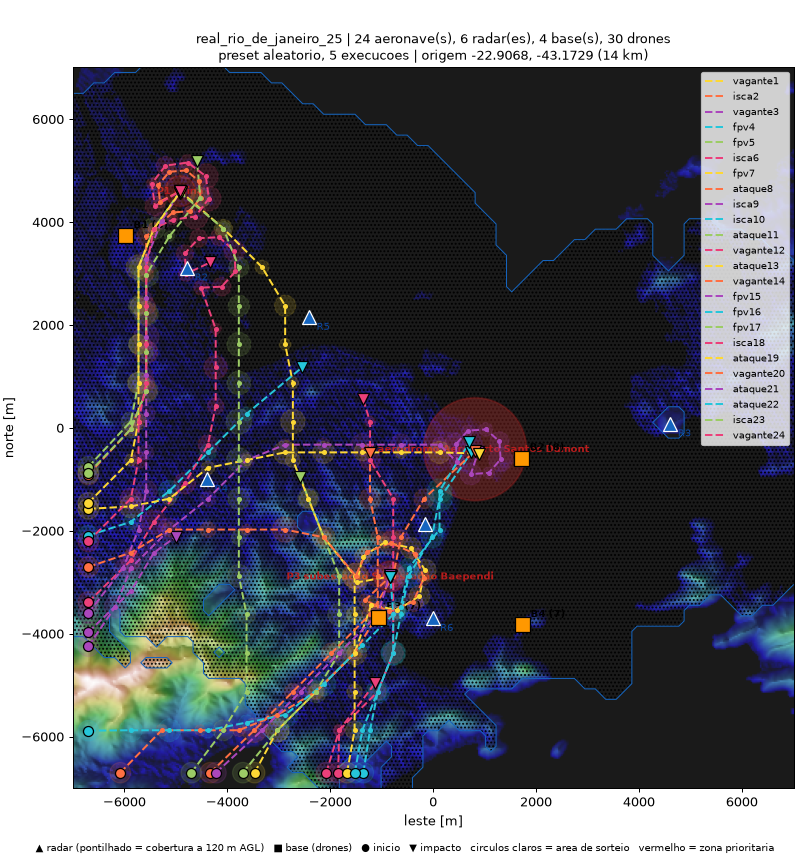
\includegraphics[width=0.75\textwidth]{figs/cenario_realista.png}
\caption{Missão de teste no Rio de Janeiro com composição equilibrada: 24 ameaças (6 de cada classe) entrando pelo setor
sudoeste, em rotas tracejadas que seguem o relevo e terminam nos impactos ($\blacktriangledown$); as munições vagantes
orbitam os alvos antes de mergulhar. Três ativos defendidos (vermelho), entre eles o aeroporto Santos Dumont; seis
radares nos morros ($\blacktriangle$, com a cobertura a 120~m sobre o terreno em pontilhado) e quatro bases com 30
interceptadores ($\blacksquare$).}
\label{fig:cenario}
\end{figure}
